% Chapter Template

\chapter{Implementation Details} % Main chapter title

\label{Chapter5} % Change X to a consecutive number; for referencing this chapter elsewhere, use \ref{ChapterX}

\lhead{Chapter 5. \emph{Implementation Details}} % Change X to a consecutive number; this is for the header on each page - perhaps a shortened title

The model overview is shown below. The EEG data from the MAHNOB-HCI datatset is passed through the pipeline.

\begin{figure}[H]
\centering
% \hspace*{-1.5cm}
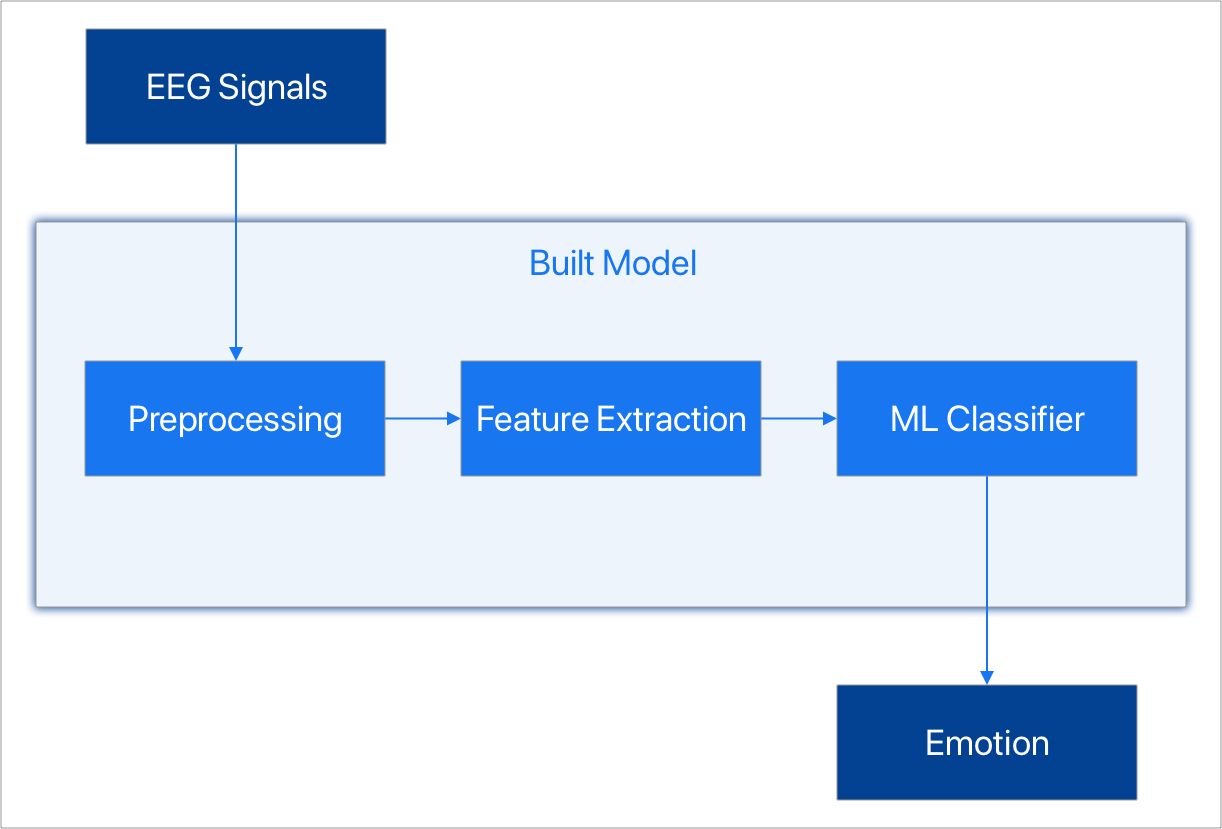
\includegraphics[height=9cm]{Figures/built_model.png}
\caption{Model Overview}
\label{fig22}
\end{figure}

\section{Preprocessing}

\begin{figure}[H]
\hspace*{-0.7cm}
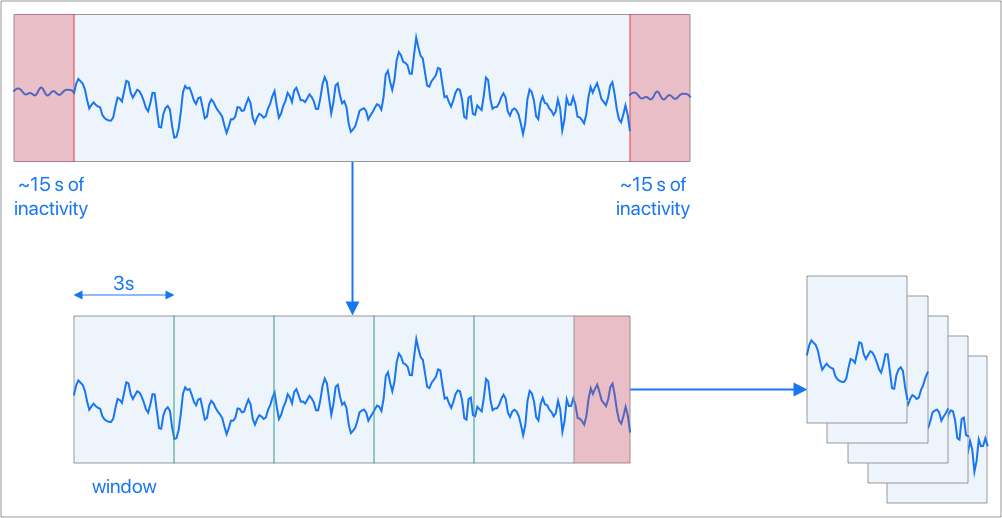
\includegraphics[height=8cm]{Figures/preprocess.png}
\caption{Preprocessing Steps}
\label{fig23}
\end{figure}

\begin{enumerate}
\item Each BDF file was read using the MNE toolkit.
\item The start time \texttt{start} and end time \texttt{end} of the video was read from the Status channel.
\item The data in between these intervals, \texttt{data[start:end]}, was cropped out and converted to a DataFrame.
\item A window size, \texttt{win\_size} (in seconds), which can be controlled externally, was defined. The default value was 3.
\item Simple signal preprocessing techniques like baseline removal and standardization can be used. The options can be tweaked while running the script \texttt{preprocess.py}.
\item The \texttt{data[start:end]} was divided into chunks of \texttt{win\_size} seconds. The last chunk was dropped if its duration was lesser than \texttt{win\_size}. The sampling frequency of the dataset is 256 Hz. Hence, each chunk, \texttt{epoch}, was of size \texttt{32}\times(\texttt{256} * \texttt{win\_size}).
\end{enumerate}

\section{Feature Extraction}
\label{sec:featureExtraction}

\begin{figure}[H]
\centering
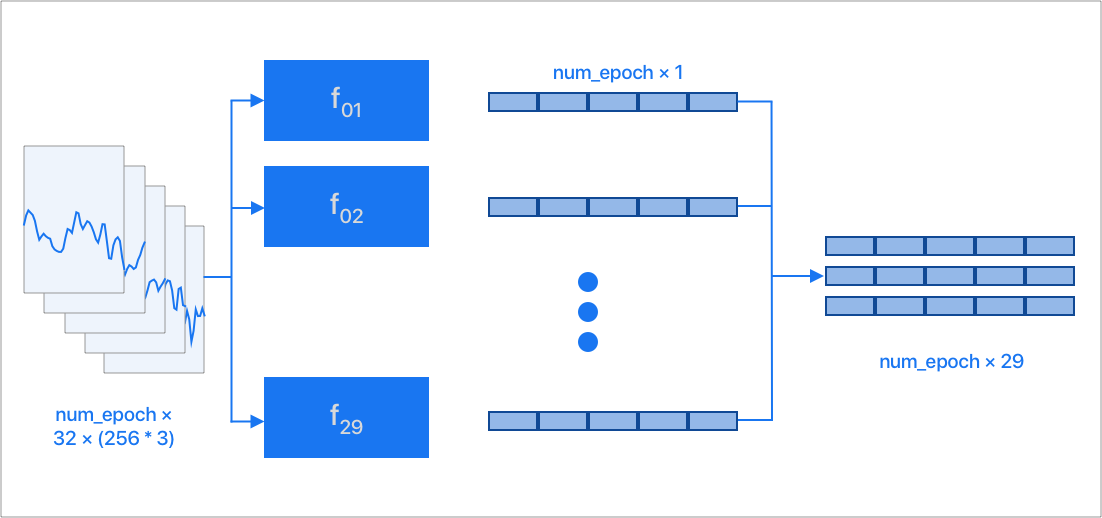
\includegraphics[height=7cm]{Figures/feat_extract.png}
\caption{Feature Extraction Pipeline}
\label{fig23}
\end{figure}

29 features were extracted from every \texttt{winsize} seconds window for all the 32 channels, resulting in a total $29 * 32 = 928$ features for every \texttt{epoch}. The features extracted from each channel are described below:
\begin{enumerate}

\item \emph{Coefficient of Variation}: The ratio of the mean of a distribution to its variance is known as its coefficient of variation. It measures how dispersed the distribution is.
\begin{tightcenter}
$C_{v}=\dfrac {\sigma }{\mu }$
\end{tightcenter}

\item \emph{Kurtosis}: The sharpness of the tail of a distribution is measured by its Kurtosis. How heavy the tail is, or how much data is aggregated at the extremities is measured using this. It is measured by calculating the ratio between the fourth central moment and the standard deviation raised to its fourth power.
\begin{tightcenter}
$\text{Kutosis} = E\left[ \left( \dfrac {X-\mu }{\sigma }\right) ^{4}\right]
 = \dfrac{\mu_4}{\sigma^4}$
\end{tightcenter}

\item \emph{Skew}: The asymmetry of a distribution, i.e., how heavy one side of a distribution is as compared to another, or how much the distribution varies from a uniform (and symmetrical distribution) is calculated using this measure.
\begin{tightcenter}
$\text{Skew} = {E\left[ \left( \dfrac {X-\mu }{\sigma }\right) ^{4}\right]} = {\dfrac {\kappa_{3}}{\kappa_{2}^{3/2}}}$,
\end{tightcenter}
where ${\kappa_i = \dfrac {1}{N}\sum ^{N}_{n=1}\left( x\left[ n\right] -\overline {x}\right) ^{i}}$ is the sample \texttt{ith} central moment.

\item \emph{First and Second Order Discrete Difference}: Given the sequence ${S_0 = [s_0^0, s_0^1, \ldots s_0^n]}$, ${S_1}$ is defined as ${S_1 = [s_1^0, s_1^1, \ldots s_1^{n-1}]}$, where $s_1^i = (s_0^{i + 1} - s_0^i)$. So the general $ith$ order discrete difference is calculated by
\begin{tightcenter}
$S_k = [s_k^0, s_k^1, \ldots s_k^{n - k}]$, where $s_k^i = (s_{k-1}^{i + 1} - s_{k - 1}^i)$.
\end{tightcenter}

\item \emph{Autoregressive Parameters using Burg's Method}: A statistical model which predicts the output at a particular time by taking into account the outputs in the previous time steps (as input to the model), is called an autoregressive model. An AR model of order $p$ can be described as:
\begin{tightcenter}
$F(x_t, [y_{t - p}, y_{t - p + 1}, \ldots, y_{t - 1}]) = y_{t}^{\prime}$.
\end{tightcenter}
Formally, the parameters of an AR model is mathematically defined as:
\begin{tightcenter}
${F_{t}=c+\sum _{{i=1}}^{p}\varphi _{i}F_{{t-i}}+\varepsilon _{t}}$,
\end{tightcenter}
where $\varphi _{i}$ are the parameters of the AR model.
\item \emph{Hjorth Parameters}: Hjorth Parameters are some statistical measures related to a time-series. This statistical measure is commonly used in EEG signal analysis. Introduced by Bo Hjorth, there are three parameters in this measure : Activity, Mobility and Complexity.
\begin{tightcenter}
${\displaystyle {\text{Activity}}={\text{var}}(f(t)).}$
\end{tightcenter}
\begin{tightcenter}
${\displaystyle {\text{Mobility}}={\sqrt {\frac {{\text{var}}({\frac {df(t)}{dt}})}{{\text{var}}(f(t))}}}.}$
\end{tightcenter}
\begin{tightcenter}
${\displaystyle {\text{Complexity}}={\frac {{\text{Mobility}}({\frac {df(t)}{dt}})}{{\text{Mobility}}(f(t))}}.}$
\end{tightcenter}
\item \emph{Power Spectral Density using Welch's Method}: Welch's method is an estimator for power spectral density. The brief overview of the steps: 
\begin{enumerate}
    \item The input signal is sliced up into $S$ segments of some window size $W$. The window overlaps by $V$ points.
    \item The overlapping $S$ segments are then tapered using a Gaussian or sinusoidal filter, giving more weightage to the center than at the ends.
    \item The periodogram is taken by using discrete FTT, and calculating its square. The average of all the periodograms are taken and hence, the resultant frequency series of the signal is generally quite smooth as compared to a Full FFT of the complete signal.
\end{enumerate}

\item \emph{Wavelet Features}: A Fourier Transform has a big disadvantage: the transformed signals have no temporal information at all, i.e., if a particular frequency is high, there is no way of confirming whether the appeared continuously, or appeared in short bursts. one solution could STFT. However, Wavelet Transform goes beyond STFT.

Wavelet Transformation on a wave performs better analysis than STFT. It multiplies the signal by a window function and performs an orthogonal expansion, like other linear integral transformations. There are two major differences as compared to STFT:
\begin{enumerate}
    \item The basis functions, known as wavelets, are way more complicated than the sinusoidal waves used in Fourier transform.
    \item The analysis ocuurs at multiple scales.
\end{enumerate}
Wavelets provide a localization in time (space) to a certain degree. However, there is always some loss due to Heisenberg's uncertainty principle. Some commonly used wavelets are:
\begin{enumerate}
    \item Haar
    \item Meyer
    \item Morlet
    \item Daubechies-4
    \item Mexican hat
\end{enumerate}
\end{enumerate}
This feature extraction step was controlled by another parameter. The user might want to average out the feature values from the 32 channels. In that case number of features outputted for each epoch was $29$ and not $928$.

\begin{figure}[H]
\centering
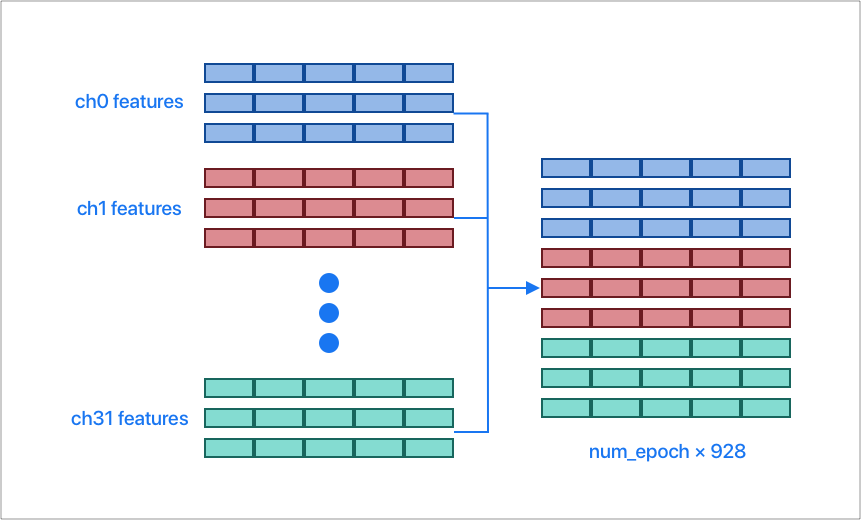
\includegraphics[height=7cm]{Figures/feat_channel_concat.png}
\caption{Features from all channels appended}
\label{fig23}
\end{figure}

\begin{figure}[H]
\centering
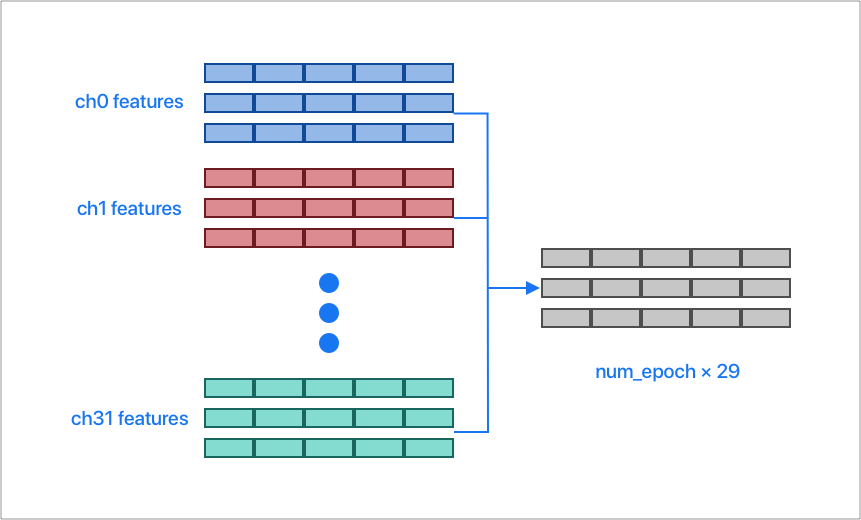
\includegraphics[height=7cm]{Figures/feat_channel_avg.png}
\caption{Features from all channels averaged}
\label{fig23}
\end{figure}

\section{Classification Model}

The features extracted from the \hyperref[sec:featureExtraction]{previous section} 32 channels along with the 4 labels (\textbf{valence}, \textbf{arousal}, \textbf{control} and \textbf{prediction}) for each epoch are now fed into machine learning models to perform the classification task.

\begin{figure}[H]
\hspace*{-1.5cm}
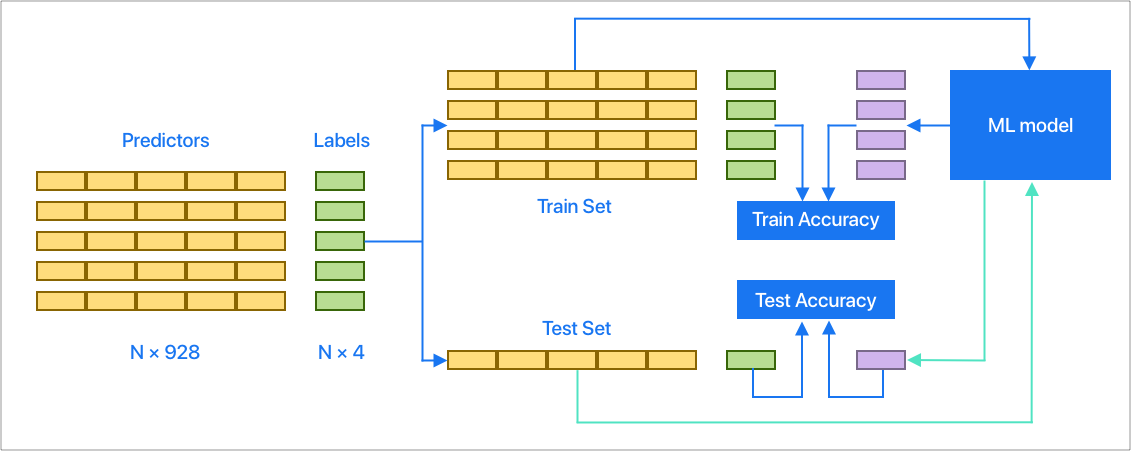
\includegraphics[height=7cm]{Figures/train_test.png}
\caption{Classification Model}
\label{fig23}
\end{figure}

The process of producing the train and test set from the input data is described below:
\begin{enumerate}
    \item The link to data stored as a DataFrame (saved in \texttt{pickle} format) in provided by the user. It is read as \texttt{df}.
    \item The fraction of the data to be used for testing (\texttt{test\_frac}) can be supplied as input by the user. By default, this value is 0.2.
    \item The rows containing non-numeric (\texttt{NaN}) values are dropped, and the complete table is shuffled by rows. Here, each row is a single data point.
    \item The mode of division of datatype can be either \textbf{random} or by \textbf{subjectid}, which can also be configured by the user. By default, the data is split randomly.
    \begin{enumerate}
        \item In case the division is random, the initial \texttt{test\_frac} portion of data is made test\_set, while the remaining part is made train\_set.
        \item In case the division is using subjectid: first the unique subjectids are extracted from the table, the ids are shuffled randomly, the initial \texttt{test\_frac} fraction of subjectids are assigned to test\_set, while the remaining are assigned to train\_set.
    \end{enumerate}
    \item After getting the train and test sets, each set is split into \texttt{X} and \texttt{Y}.
    \begin{enumerate}
        \item The feature vector (size 928), \texttt{X}, and the raw label values (size 4, values ranging in \texttt{[1 - 9]}), \texttt{Y\_raw}, are extracted as columns, split from \texttt{t-set}, which can be train or test set.
        \item The number of classes \texttt{num\_classes} into which the raw labels, \texttt{Y\_raw}, are to be divided can be configured by the user. By default this value is 3.
        \item The raw label values are binned into \texttt{num\_classes}, and is named \texttt{Y}. So, finally the values in the labels are in the range \texttt{0 - num\_classes}
    \end{enumerate}
    \item For each of the 4 labels (\textbf{V}alence, \textbf{A}rousal, \textbf{C}ontrol and \textbf{P}rediction, the column \texttt{y} is extracted as the label, and 928 columns are used as rows for training an ML model.
    \item The type of model on which the data is to be trained is also configurable by the user. Currently, Random Forest and XGBoost have been used as they are one of the best ML models using bagging and boosting methods, respectively, and are used actively in research.
    \item The performance metrics and feature importance of the trained model are calculated and plotted finally.
\end{enumerate}

\begin{figure}[H]
\centering
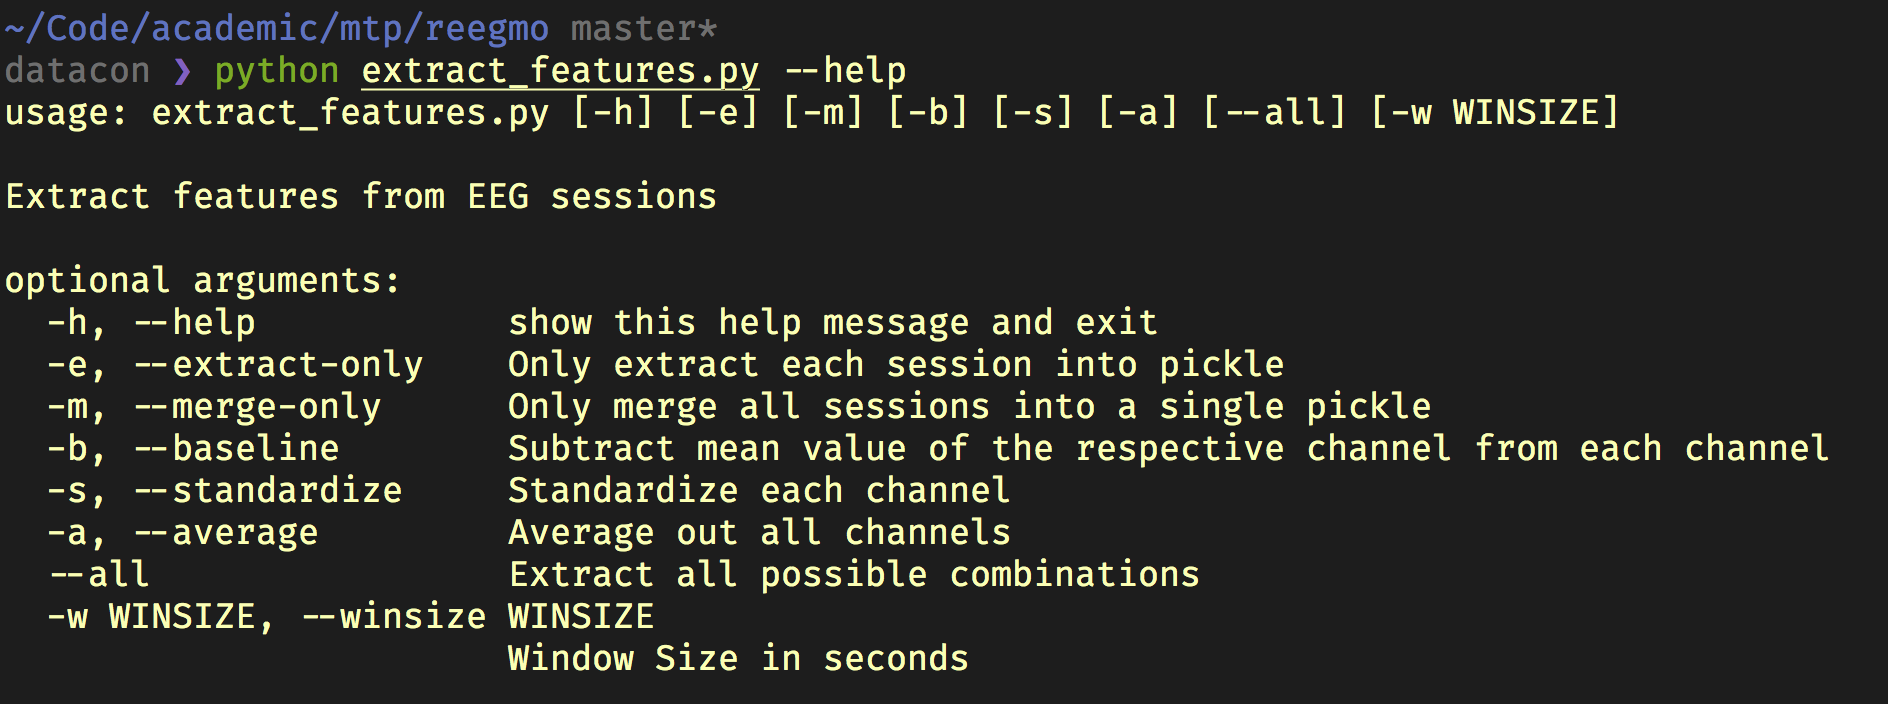
\includegraphics[height=5cm]{Figures/extract_features_help.png}
\caption{\texttt{extract\_features}}
\label{fig23}
\end{figure}

\begin{figure}[H]
\centering
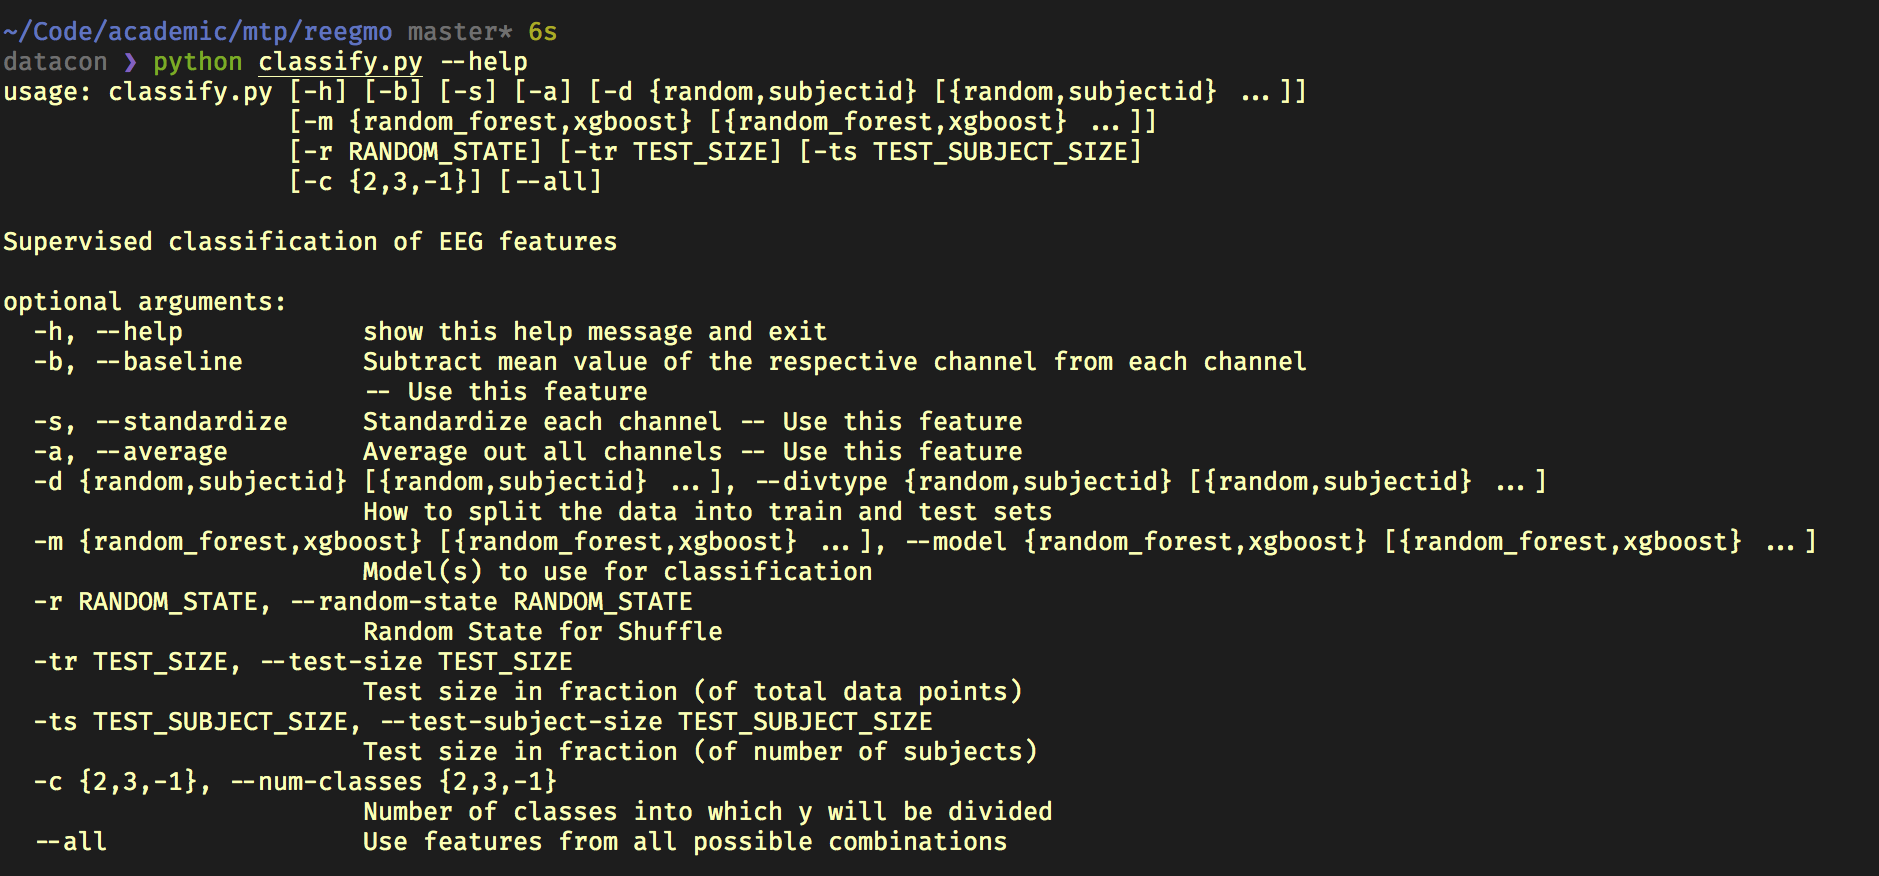
\includegraphics[height=6.2cm]{Figures/classify_help.png}
\caption{\texttt{classify}}
\label{fig23}
\end{figure}
